\documentclass[aspectratio=169]{beamer}
\usepackage[style=ieee,backend=biber]{biblatex}
    \addbibresource{reference.bib}
\usepackage{colortbl,tabularx,mathrsfs,calligra}
\usepackage{amsmath,amsfonts,amssymb,amsthm}
\usepackage{ragged2e}
\usepackage[bahasa]{babel}
\usepackage{tikz}
\usepackage{caption}
\usepackage{wrapfig}
\usepackage{multirow}
\usepackage{multicol}
\usepackage{array}
\usepackage{pgfplots, tkz-euclide,calc}
    \pgfplotsset{compat=1.18}
\usepackage{listings}

\graphicspath{{C:/Users/teoso/OneDrive/Documents/Tugas Kuliah/Template Math Depart/}{./foto/}}

\definecolor{HIMAmuda}{HTML}{01D1FD}
\definecolor{HIMAtua}{HTML}{02016A}
\definecolor{HIMAabu}{HTML}{CBCBCC}

\usetheme{Madrid}

\setbeamercolor{palette primary}{bg=HIMAtua,fg=white}
\setbeamercolor{palette secondary}{bg=HIMAmuda,fg=black}
\setbeamercolor{palette tertiary}{bg=HIMAabu,fg=black}
\setbeamercolor{palette quaternary}{bg=HIMAmuda,fg=white}
\setbeamercolor{structure}{fg=HIMAmuda} % itemize, enumerate, etc
\setbeamercolor{section in toc}{fg=HIMAtua} % TOC sections
\setbeamercolor{bibliography item}{parent=palette secondary}
\setbeamercolor*{bibliography entry author}{parent=section in toc}

\usetikzlibrary{shapes.geometric, arrows}

\tikzstyle{startstop} = [ellipse, minimum width=1cm, minimum height=1cm,text centered, draw=black, fill=red!30]
\tikzstyle{process} = [rectangle, minimum width=2cm, minimum height=1cm, text centered, draw=black, fill=blue!30]
\tikzstyle{decision} = [diamond, minimum width=1cm, minimum height=1cm, text centered, draw=black, fill=blue!50]
\tikzstyle{arrow} = [thick,->,>=stealth]

\newcolumntype{L}[1]{>{\raggedright\let\newline\\\arraybackslash\hspace{0pt}}m{#1}}
\newcolumntype{C}[1]{>{\centering\let\newline\\\arraybackslash\hspace{0pt}}m{#1}}
\newcolumntype{R}[1]{>{\raggedleft\let\newline\\\arraybackslash\hspace{0pt}}m{#1}}

\usefonttheme{professionalfonts}
\setbeamertemplate{theorems}[numbered]
\setbeamertemplate{bibliography item}{\insertbiblabel}
% \setbeamercovered{transparent}


\theoremstyle{definition}
% \numberwithin{subsection}{section}
\newtheorem{definisi}{Definisi}
\numberwithin{definisi}{subsection}
\newtheorem{teorema}[definisi]{TEOREMA}
\newcommand{\R}{\mathbb{R}}
\newcommand{\N}{\mathbb{N}}
\newcommand{\Z}{\mathbb{Z}}
\newcommand{\C}{\mathbb{C}}


\AtBeginEnvironment{contoh}{%
  \setbeamercolor{block title}{use=example text,fg=white,bg=example text.fg!75!black}
  \setbeamercolor{block body}{parent=normal text,use=block title example,bg=block title example.bg!10!bg}
}
\AtBeginEnvironment{definisi}{
    \setbeamercolor{block title}{fg=white,bg=HIMAtua}
    \setbeamercolor{block body}{parent=normal text,bg=HIMAtua!30!white}
}

\date{Jum'at, 6 Desember 2024}
\title[Proposal TA]{Model Penjadwalan Suroboyo Bus Menggunakan Aljabar Max-Plus}
\author[Teo]{Teosofi Hidayah Agung}
\institute[Matematika ITS]{Departemen Matematika\\ Institut Teknologi Sepuluh Nopember}
\titlegraphic{
\includegraphics[scale=0.15]{logoITS}$\quad$
\includegraphics[scale=0.024]{M.png}}

\begin{document}
    \begin{frame}
        \titlepage
    \end{frame}

\AtBeginSection[]
{
    \begin{frame}{Daftar isi}
        \tableofcontents[currentsection,hidesubsections]
    \end{frame}
}

    \section{Pendahuluan}
    \subsection{Latar Belakang}
    \begin{frame}
        \frametitle{\insertsubsection}
        \begin{figure}
            \centering
            \onslide<2->{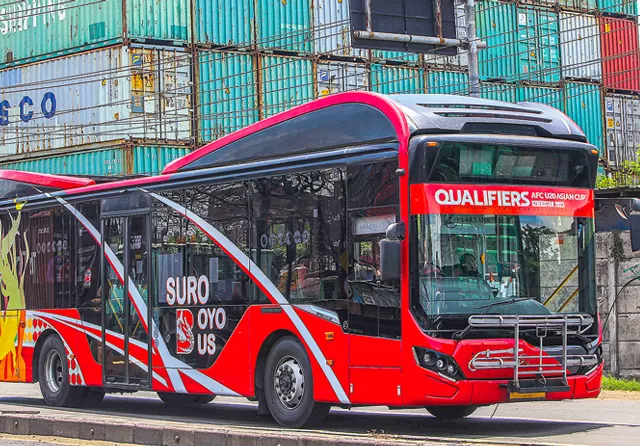
\includegraphics[width=0.3\textwidth]{Suroboyo bus.png}$\quad\quad$}
            \onslide<3->{{\caption{Suroboyo Bus \cite{jawapos2024suroboyobus}}}}
        \end{figure}
        \onslide<3->{Suroboyo bus adalah fasilitas publik yang disediakan oleh Pemerintah Kota Surabaya yang beroperasi dibeberapa rute krusial di Surabaya. Pada awalnya transportasi ini adalah upaya Pemerintah untuk mengurangi sampah plastik, namun sekarang telah dialihfungsikan menjadi salah satu transportasi dengan tarif yang cukup murah.}
    \end{frame}

    \begin{frame}
        \frametitle{\insertsubsection}
        Berdasarkan penelitian yang dilakukan \citeauthor{primadhanny2023pengaruhsuroboyobus}, didapatkan bahwa tingkat kepuasan penumpang terhadap Suroboyo Bus mencapai 77,49\%. Hal ini dapat menjadi pertimbangan bagi Pemerintah Kota Surabaya untuk terus mengembangkan Suroboyo Bus agar dapat memberikan pelayanan yang lebih baik lagi.
    \end{frame}

    \begin{frame}
        \frametitle{\insertsubsection}
        \begin{figure}
            \centering
            \onslide<2->{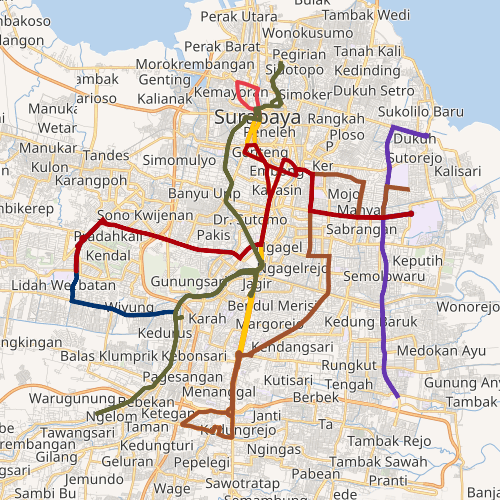
\includegraphics[width=0.25\textwidth]{rute suroboyo bus.png}$\quad$}
            \onslide<3->{\caption{Rute Suroboyo Bus \cite{wikipedia2024suroboyobus}}}
        \end{figure}
        \onslide<3->{Dapat dilihat bahwa rute Suroboyo Bus melewati beberapa terminal yang berbeda pada suatu waktu. Sehingga objek diskrit ini dapat dimodelkan dengan menggunakan representasi graf.}
    \end{frame}

    \begin{frame}
        Aljabar max-plus adalah salah satu cabang matematika yang dapat digunakan untuk memodelkan sistem jaringan transportasi. Dengan menggunakan aljabar max-plus, dapat dilakukan perencanaan jadwal keberangkatan dan kedatangan bus yang optimal.

        Penelitian serupa juga telah dilakukan oleh \citeauthor{AfwanGiri2023PemodelanMaxPlus} yang dimana mereka memodelkan penjadwalan bus untuk Bus Trans Semarang.
    \end{frame}

    \subsection{Rumusan Masalah}
    \begin{frame}
        \frametitle{\insertsubsection}
        \begin{enumerate}
            \item \onslide<2->{Bagaimana memodelkan rute lalu lintas Suroboyo Bus menggunakan graf berarah dan berbobot?}
            \item \onslide<3->{Bagaimana penerapan aljabar max-plus dalam perencanaan jadwal kedatangan dan keberangkatan Suroboyo Bus?}
        \end{enumerate}
    \end{frame}

    \subsection{Batasan Masalah}
    \begin{frame}
        \frametitle{\insertsubsection}
        \begin{itemize}
            \item \onslide<2->{Data dikumpulkan dari data Dishub  atau secara mandiri melalui observasi lapangan dengan menaiki bus.}
            \item \onslide<3->{Hanya jadwal kedatangan dan keberangkatan bus yang akan dianalisis, tanpa mempertimbangkan faktor eksternal seperti cuaca, kondisi jalan, atau perubahan kebijakan transportasi.}
            \item \onslide<4->{Rute yang akan dianalisis adalah rute yang jalurnya masih berada dilingkungan kampus ITS, yakni Koridor R2, Koridor R4, dan Koridor SBT.}
        \end{itemize}
    \end{frame}

    \subsection{Tujuan}
    \begin{frame}
        \frametitle{\insertsubsection}
        \begin{enumerate}
            \item \onslide<2->{Memodelkan rute lalu lintas Suroboyo Bus menggunakan graf berarah dan berbobot.}
            \item \onslide<3->{Mengoptimalkan jadwal operasional bus di terminal untuk meminimalkan waktu tunggu penumpang.}
        \end{enumerate}
    \end{frame}

    \subsection{Manfaat}
    \begin{frame}
        \frametitle{\insertsubsection}
        \begin{itemize}
            \item \onslide<2->{\textbf{Manfaat Teoritis}: Memberikan kontribusi pada pengembangan ilmu pengetahuan, khususnya dalam bidang transportasi dan matematika terapan melalui penerapan aljabar max-plus dalam perencanaan jadwal transportasi umum.}
            \item \onslide<3->{\textbf{Manfaat Praktis}: Menjadikan pertimbangan Pemerintah kota Surabaya terhadap Suroboyo Bus mengoptimalkan jadwal keberangkatan dan kedatangan bus sehingga dapat meningkatkan efisiensi operasional.}
        \end{itemize}
    \end{frame}

    \section{Tinjauan Pustaka}
    \subsection{Aljabar Max-Plus}
    \begin{frame}
        \frametitle{\insertsubsection}
        \begin{definisi}[\cite{subiono2015minmaxplus}]
            Aljabar max-plus adalah suatu semiring di $\R \cup \{\varepsilon=-\infty\}$ dengan dua operasi biner yaitu
            \begin{align*}
                a \oplus b &= \max\{a,b\},\\
                a \otimes b &= a + b.
            \end{align*}
        \end{definisi}
        \onslide<2->{Misal: $a = 3, b = 5$, maka
            \begin{align*}
                a \oplus b &= \max\{3,5\} = 5,\\
                a \otimes b &= 3 + 5 = 8.
            \end{align*}}
    \end{frame}

    \subsection{Vektor dan Matriks}
    \begin{frame}
        \frametitle{\insertsubsection}
        \begin{definisi}[\cite{butkovic2010maxplus}]
            Misalkan $A$ adalah matriks $n \times n$ dengan elemen $a_{ij} \in \R \cup \{\varepsilon\}$, maka vektor $x$ adalah vektor kolom dengan elemen $x_i \in \R \cup \{\varepsilon\}$, dan perkalian matriks-vektor didefinisikan sebagai
            \[
                A\otimes x = \max_{j=1}^{n} \{a_{ij} + x_j\}.
            \]
        \end{definisi}
        \onslide<2->{Misal: $A = \begin{pmatrix} 1 & 2 \\ 3 & 4 \end{pmatrix}$, $x = \begin{pmatrix} 5 \\ 6 \end{pmatrix}$, maka
            \[
                A\otimes x = \begin{pmatrix} \max\{6,8\} \\ \max\{8,10\} \end{pmatrix} = \begin{pmatrix} 8 \\ 10 \end{pmatrix}.
            \]}
    \end{frame}

    \subsection{Graf Aljabar Max-Plus}
    \begin{frame}
        \frametitle{\insertsubsection}
        Misalkan graf $\mathcal{G}$ adalah graf berarah berbobot seperti yang diilustrasikan
        \begin{center}
            \begin{tikzpicture}[node distance=1.5cm, auto, >=stealth]
                \node[circle, draw, fill=blue!20] (A) at (0, 0) {P};
                \node[circle, draw, fill=blue!20] (C) at (4, 0) {Q};
                \draw[->, thick] (A) to[bend left] node[midway, above] {3} (C);
                \draw[->, thick] (C) to[bend left] node[midway, below] {5} (A);
                \draw[->, thick] (C) to[loop right] node[midway, right] {1} (C);
            \end{tikzpicture}
        \end{center}
        \onslide<2->{Matriks representasi dari graf $\mathcal{G}$ adalah
            \[
                A = \begin{pmatrix} a_{11} & a_{12} \\ a_{21} & a_{22} \end{pmatrix} = \begin{pmatrix} \varepsilon & 5 \\ 3 & 1 \end{pmatrix}.
            \]}
    \end{frame}

    \subsection{Nilai Eigen dan Vektor Eigen}
    \begin{frame}
        \frametitle{\insertsubsection}
        \begin{definisi}[\cite{baccelli}]
            Misalkan $A$ adalah matriks $n \times n$ dengan elemen $a_{ij} \in \R \cup \{\varepsilon\}$, maka nilai eigen dari $A$ adalah bilangan $\lambda \in \R \cup \{\varepsilon\}$ yang memenuhi
            \[
                A\otimes x = \lambda \otimes x.
            \]
        \end{definisi}
        \onslide<2->{Misal: $A = \begin{pmatrix} \varepsilon & 3 \\ 5 & 1 \end{pmatrix}$, maka nilai eigen dari $A$ adalah $\lambda = 4$ dengan vektor eigen $x = \begin{pmatrix} 0 \\ 1 \end{pmatrix}$.}
    \end{frame}

    \subsection{SPL Aljabar Max-Plus}
    \begin{frame}
        \frametitle{\insertsubsection}
        Kembali pada graf $\mathcal{G}$
        \begin{center}
            \begin{tikzpicture}[node distance=1.5cm, auto, >=stealth]
                \node[circle, draw, fill=blue!20] (A) at (0, 0) {P};
                \node[circle, draw, fill=blue!20] (C) at (4, 0) {Q};
                \draw[->, thick,] (A) to[bend left] node[midway, above] {3} (C);
                \draw[->, thick,] (C) to[bend left] node[midway, below] {5} (A);
                \draw[->, thick,] (C) to[loop right] node[midway, right] {1} (C);
                \onslide<3->{\draw[->, thick,blue] (C) to[bend left] node[midway, below] {5} (A);}
                \onslide<4->{\draw[->, thick,red] (A) to[bend left] node[midway, above] {3} (C);
                \draw[->, thick,red] (C) to[loop right] node[midway, right] {1} (C);}
            \end{tikzpicture}
        \end{center}
        \onslide<2->{Misalkan $y_p(k)$ dan $y_q(k)$ menunjukkan waktu keberangkatan ke-$k+1$ dari masing-masing terminal $P$ dan $Q$, maka dapat dibuat sistem pertidaksamaan yang merepresentasikan graf $\mathcal{G}$}
        \begin{columns}
            \onslide<3->{\color{blue}\column{0.5\textwidth}
            \begin{align*}
                y_p(k+1) &\geq y_p(k)\\
                y_p(k+1) &\geq y_q(k) + 5
            \end{align*}}
            \onslide<4->{\column{0.5\textwidth}{\color{red}
            \begin{align*}
                y_q(k+1) &\geq y_q(k)+1\\
                y_q(k+1) &\geq y_p(k) + 3
            \end{align*}}}
        \end{columns}
    \end{frame}

    \begin{frame}
        \frametitle{\insertsubsection}
        Dengan aturan bahwa bus harus segera berangkat setelah "diperbolehkan", maka didapatkan SPL sebagai berikut    
        \onslide<2->{\begin{align*}
            y_p(k+1) &= \max\{y_p(k), y_q(k) + 5\}\\
            y_q(k+1) &= \max\{y_q(k)+1, y_p(k) + 3\}
        \end{align*}}
        \onslide<3->{Jika ditulis dalam bentuk matriks}
        \onslide<3->{\[
        \begin{pmatrix}
            y_p(k+1)\\
            y_q(k+1)
        \end{pmatrix}= \begin{pmatrix}
            \varepsilon & 5\\
            3 & 1
        \end{pmatrix} \otimes \begin{pmatrix}
            y_p(k)\\
            y_q(k)
        \end{pmatrix}
        \]}
    \end{frame}

    \subsection{Algoritma Power}
    \begin{frame}
        \frametitle{\insertsubsection}
        Algoritma ini terdiri dari langkah-langkah berikut: 
        \begin{enumerate}
             \item Berikan nilai awal \( x(0) \neq (\varepsilon, \varepsilon, \dots, \varepsilon)^T \).
                \item Iterasikan persamaan rekursif hingga terjadi perilaku periodik \( x(p) = c \otimes x(q) \), dengan \( p > q \geq 0 \).
                \item Hitung nilai eigen \( \lambda = \frac{c}{p-q} \).
                \item Tentukan vektor eigen menggunakan:
                \[
                v = \bigoplus_{i=1}^{p-q} \left( \lambda^{p-q-i} \otimes x(q+i-1) \right).
                \]
        \end{enumerate}
    \end{frame}
    
    \section{Metodologi}
    \begin{frame}
        \frametitle{Langkah-Langkah Penelitian}
        \begin{enumerate}
            \item \onslide<2->{Memperloleh data-data yang diperlukan
            \begin{itemize}
                \item Banyaknya bus yang beroperasi
                \item Waktu keberangkatan dan kedatangan
                \item Jarak dan waktu tempuh untuk setiap rute
            \end{itemize}}
            \item \onslide<3->{Identifikasi Sistem Jaringan Suroboyo Bus}
            \item \onslide<4->{Modelkan sistem dalam graf berarah dan berbobot}
            \item \onslide<5->{Formulasikan sistem dalam aljabar max-plus}
            \item \onslide<6->{Selesaikan Model sistem dengan bantuan \textit{software Scilab}}
            \item \onslide<7->{Mendesain penjadwalan Suroboyo Bus}
        \end{enumerate}
    \end{frame}
    % \begin{frame}
    %     \begin{tikzpicture}[node distance=3cm, font=\scriptsize]

    %         % Nodes
    %         \node (start) [startstop] {Mulai};
    %         \node (data) [process, right of=start] {\parbox{1.5cm}{Identifikasi Data Awal}};
    %         \node (formulasi) [process, right of=data] {\parbox{2.5cm}{Formulasi Sistem dalam Aljabar Max-Plus}};
    %         \node (dinamika) [process, right of=formulasi] {\parbox{1.5cm}{Modeling Dinamika Jadwal}};
    %         \node (validasi) [process, right of=dinamika] {\parbox{1.5cm}{Analisis Validitas Model}};
    %         \node (optimasi) [process, below of=validasi] {Optimasi Jadwal};
    %         \node (evaluasi) [decision, left of=optimasi] {\parbox{1.5cm}{Evaluasi dan Validasi}};
    %         \node (implementasi) [process, left of=evaluasi] {\parbox{2cm}{Implementasi dan Simulasi}};
    %         \node (kesimpulan) [process, left of=implementasi] {\parbox{2cm}{Kesimpulan dan Dokumentasi}};
    %         \node (end) [startstop, left of=kesimpulan] {Selesai};
            
    %         % Arrows
    %         \draw [arrow] (start) -- (data);
    %         \draw [arrow] (data) -- (formulasi);
    %         \draw [arrow] (formulasi) -- (dinamika);
    %         \draw [arrow] (dinamika) -- (validasi);
    %         \draw [arrow] (validasi) -- (optimasi);
    %         \draw [arrow] (optimasi) -- (evaluasi);
    %         \draw [arrow,red] (evaluasi) -- node[midway,above left]{no} ++(0,1.5) -| (formulasi);
    %         \draw [arrow,green] (evaluasi) --node[midway,above]{yes} (implementasi);
    %         \draw [arrow] (implementasi) -- (kesimpulan);
    %         \draw [arrow] (kesimpulan) -- (end);
    %     \end{tikzpicture}
    % \end{frame}

    % \begin{frame}
    %     \begin{table}
    %         \caption{Jadwal Kegiatan}
    %         \centering
    %         \begin{tabular}{|C{0.6cm}|L{5.7cm}|C{0.25cm}|C{0.25cm}|C{0.25cm}|C{0.25cm}|C{0.25cm}|C{0.25cm}|C{0.25cm}|C{0.25cm}|C{0.25cm}|C{0.25cm}|C{0.25cm}|C{0.25cm}|}
    %         \hline
    %         &&\multicolumn{12}{c|}{\textbf{BULAN}}\\\cline{3-14}
    %         \multicolumn{1}{|c|}{\textbf{NO}}&\multicolumn{1}{c|}{\textbf{NAMA KEGIATAN}}&\multicolumn{4}{c|}{1}&\multicolumn{4}{c|}{2}&\multicolumn{4}{c|}{3}\\\cline{3-14}
    %         &&1&2&3&4&1&2&3&4&1&2&3&4\\\cline{1-14}
            
    %         1&Identifikasi Data Awal&\cellcolor{HIMAtua}&\cellcolor{HIMAtua}&&&&&&&&&&\\\hline
    %         2&Formulasi Sistem dalam Aljabar Max-Plus&&&\cellcolor{HIMAtua}&\cellcolor{HIMAtua}&\cellcolor{HIMAtua}&&&&&&&\\\hline
    %         3&Modeling Dinamika Jadwal&&&&&\cellcolor{HIMAtua}&\cellcolor{HIMAtua}&\cellcolor{HIMAtua}&&&&&\\\hline
    %         4&Analisis Validitas Model&&&&&&&&\cellcolor{HIMAtua}&\cellcolor{HIMAtua}&\cellcolor{HIMAtua}&&\\\hline
    %         5&Optimasi Jadwal&&&&&&&&\cellcolor{HIMAtua}&\cellcolor{HIMAtua}&\cellcolor{HIMAtua}&&\\\hline
    %         6&Implementasi dan Simulasi&&&&&&&&&\cellcolor{HIMAtua}&\cellcolor{HIMAtua}&\cellcolor{HIMAtua}&\\\hline
    %         7&Kesimpulan dan Dokumentasi&&&&&&&&&\cellcolor{HIMAtua}&\cellcolor{HIMAtua}&\cellcolor{HIMAtua}&\cellcolor{HIMAtua}\\\hline
            
    %         \end{tabular}
    %         \label{TabelJadwalKegiatan}
    %     \end{table}
    % \end{frame}

    \section{Referensi}
    \begin{frame}[allowframebreaks]
        \printbibliography
    \end{frame}
\end{document}